\documentclass{standalone}
\usepackage{tikz}
\usetikzlibrary{patterns}
\usetikzlibrary{positioning}
\usetikzlibrary{patterns, positioning}
\usetikzlibrary{shapes.misc}
\usepackage[outline]{contour}
\contourlength{1.5pt} 
\usepackage[sfdefault]{ClearSans}

\begin{document}
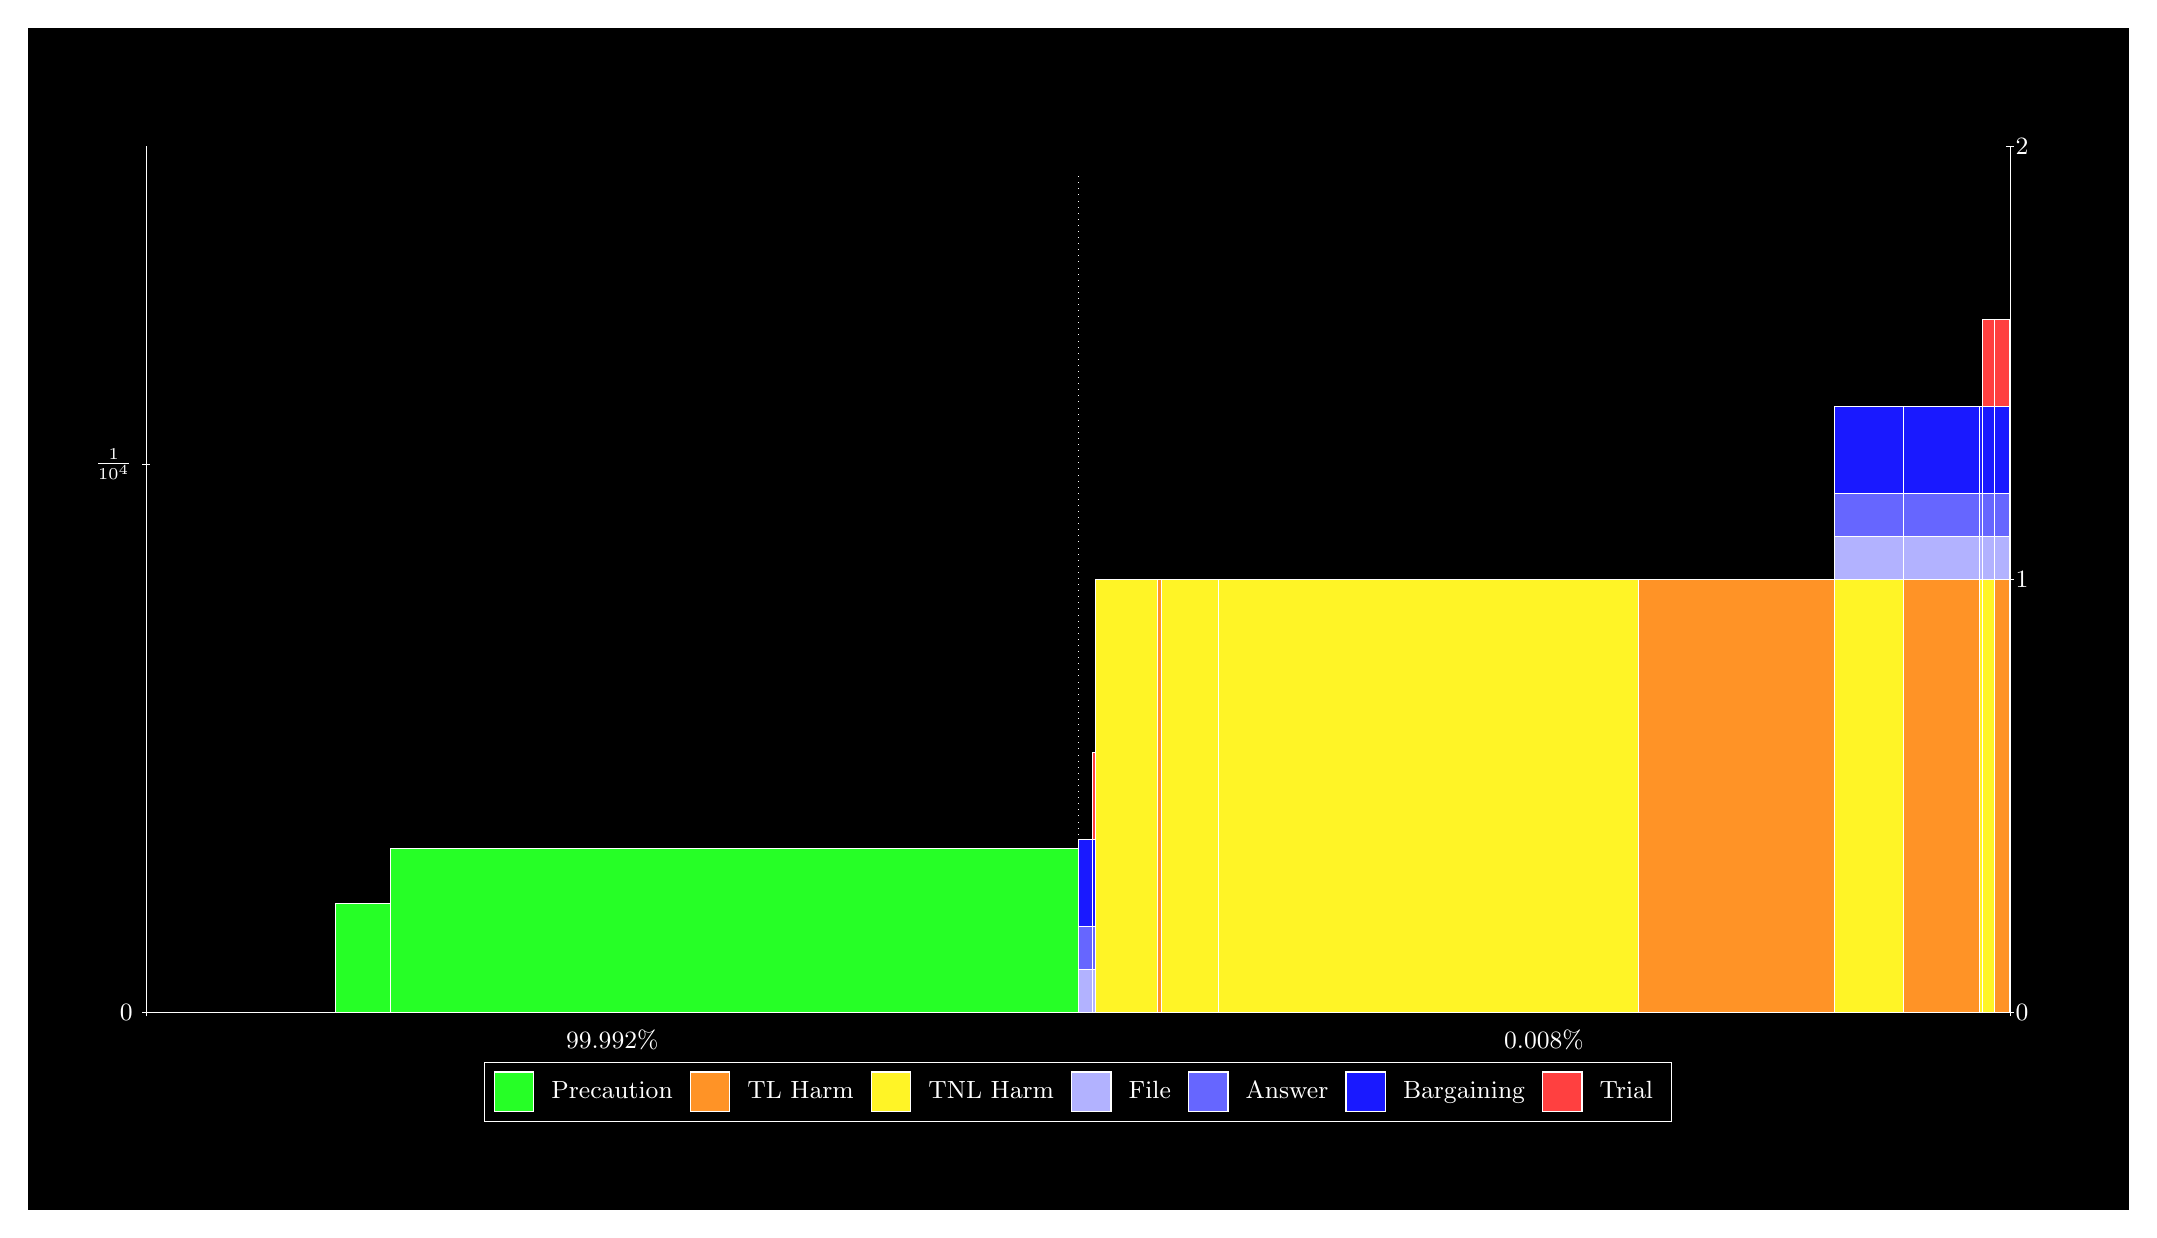
\begin{tikzpicture}
\draw[fill=black] (0,0) rectangle (26.667,15);
\draw[fill=green!85,draw=white,very thin] (3.8974,2.5) rectangle (4.597,3.8926);
\draw[fill=green!85,draw=white,very thin] (4.597,2.5) rectangle (13.333,4.5888);
\draw[fill=blue!30,draw=white,very thin] (13.333,2.5) rectangle (13.518,3.05);
\draw[fill=blue!60,draw=white,very thin] (13.333,3.05) rectangle (13.518,3.6);
\draw[fill=blue!90,draw=white,very thin] (13.333,3.6) rectangle (13.518,4.7);
\draw[fill=blue!30,draw=white,very thin] (13.518,2.5) rectangle (13.553,3.05);
\draw[fill=blue!60,draw=white,very thin] (13.518,3.05) rectangle (13.553,3.6);
\draw[fill=blue!90,draw=white,very thin] (13.518,3.6) rectangle (13.553,4.7);
\draw[fill=red!75,draw=white,very thin] (13.518,4.7) rectangle (13.553,5.8);
\draw[fill=yellow!85,draw=white,very thin] (13.553,2.5) rectangle (14.335,7.9999);
\draw[fill=orange!85,draw=white,very thin] (14.335,2.5) rectangle (14.392,7.9999);
\draw[fill=green!85,draw=white,very thin] (14.392,2.5) rectangle (15.116,2.5001);
\draw[fill=yellow!85,draw=white,very thin] (14.392,2.5001) rectangle (15.116,8);
\draw[fill=green!85,draw=white,very thin] (15.116,2.5) rectangle (20.449,2.5002);
\draw[fill=yellow!85,draw=white,very thin] (15.116,2.5002) rectangle (20.449,8.0001);
\draw[fill=green!85,draw=white,very thin] (20.449,2.5) rectangle (22.932,2.5002);
\draw[fill=orange!85,draw=white,very thin] (20.449,2.5002) rectangle (22.932,8.0001);
\draw[fill=yellow!85,draw=white,very thin] (22.932,2.5) rectangle (23.819,7.9999);
\draw[fill=blue!30,draw=white,very thin] (22.932,7.9999) rectangle (23.819,8.5499);
\draw[fill=blue!60,draw=white,very thin] (22.932,8.5499) rectangle (23.819,9.0999);
\draw[fill=blue!90,draw=white,very thin] (22.932,9.0999) rectangle (23.819,10.2);
\draw[fill=orange!85,draw=white,very thin] (23.819,2.5) rectangle (24.783,7.9999);
\draw[fill=blue!30,draw=white,very thin] (23.819,7.9999) rectangle (24.783,8.5499);
\draw[fill=blue!60,draw=white,very thin] (23.819,8.5499) rectangle (24.783,9.0999);
\draw[fill=blue!90,draw=white,very thin] (23.819,9.0999) rectangle (24.783,10.2);
\draw[fill=green!85,draw=white,very thin] (24.783,2.5) rectangle (24.814,2.5001);
\draw[fill=yellow!85,draw=white,very thin] (24.783,2.5001) rectangle (24.814,8);
\draw[fill=blue!30,draw=white,very thin] (24.783,8) rectangle (24.814,8.55);
\draw[fill=blue!60,draw=white,very thin] (24.783,8.55) rectangle (24.814,9.1);
\draw[fill=blue!90,draw=white,very thin] (24.783,9.1) rectangle (24.814,10.2);
\draw[fill=green!85,draw=white,very thin] (24.814,2.5) rectangle (24.816,2.5001);
\draw[fill=orange!85,draw=white,very thin] (24.814,2.5001) rectangle (24.816,8);
\draw[fill=blue!30,draw=white,very thin] (24.814,8) rectangle (24.816,8.55);
\draw[fill=blue!60,draw=white,very thin] (24.814,8.55) rectangle (24.816,9.1);
\draw[fill=blue!90,draw=white,very thin] (24.814,9.1) rectangle (24.816,10.2);
\draw[fill=yellow!85,draw=white,very thin] (24.816,2.5) rectangle (24.972,7.9999);
\draw[fill=blue!30,draw=white,very thin] (24.816,7.9999) rectangle (24.972,8.5499);
\draw[fill=blue!60,draw=white,very thin] (24.816,8.5499) rectangle (24.972,9.0999);
\draw[fill=blue!90,draw=white,very thin] (24.816,9.0999) rectangle (24.972,10.2);
\draw[fill=red!75,draw=white,very thin] (24.816,10.2) rectangle (24.972,11.3);
\draw[fill=orange!85,draw=white,very thin] (24.972,2.5) rectangle (25.161,7.9999);
\draw[fill=blue!30,draw=white,very thin] (24.972,7.9999) rectangle (25.161,8.5499);
\draw[fill=blue!60,draw=white,very thin] (24.972,8.5499) rectangle (25.161,9.0999);
\draw[fill=blue!90,draw=white,very thin] (24.972,9.0999) rectangle (25.161,10.2);
\draw[fill=red!75,draw=white,very thin] (24.972,10.2) rectangle (25.161,11.3);
\draw[fill=green!85,draw=white,very thin] (25.161,2.5) rectangle (25.165,2.5001);
\draw[fill=yellow!85,draw=white,very thin] (25.161,2.5001) rectangle (25.165,8);
\draw[fill=blue!30,draw=white,very thin] (25.161,8) rectangle (25.165,8.55);
\draw[fill=blue!60,draw=white,very thin] (25.161,8.55) rectangle (25.165,9.1);
\draw[fill=blue!90,draw=white,very thin] (25.161,9.1) rectangle (25.165,10.2);
\draw[fill=red!75,draw=white,very thin] (25.161,10.2) rectangle (25.165,11.3);
\draw[fill=green!85,draw=white,very thin] (25.165,2.5) rectangle (25.167,2.5001);
\draw[fill=orange!85,draw=white,very thin] (25.165,2.5001) rectangle (25.167,8);
\draw[fill=blue!30,draw=white,very thin] (25.165,8) rectangle (25.167,8.55);
\draw[fill=blue!60,draw=white,very thin] (25.165,8.55) rectangle (25.167,9.1);
\draw[fill=blue!90,draw=white,very thin] (25.165,9.1) rectangle (25.167,10.2);
\draw[fill=red!75,draw=white,very thin] (25.165,10.2) rectangle (25.167,11.3);
\draw[white,very thin] (1.5,2.5) -- (1.5,13.5);
\draw[white,very thin] (1.45,2.5) -- (1.55,2.5);
\node[font=\small,text=white, anchor=east] at (1.45, 2.5) {0};
\draw[white,very thin] (1.45,9.4628) -- (1.55,9.4628);
\node[font=\small,text=white, anchor=east] at (1.45, 9.4628) {$\frac{1}{10^{4}}$};

\draw[white,dotted,very thin] (13.333,2.83) -- (13.333,13.17);
\draw[white,very thin] (25.167,2.5) -- (25.167,13.5);
\draw[white,very thin] (25.117,2.5) -- (25.217,2.5);
\node[font=\small,text=white, anchor=west] at (25.117, 2.5) {0};
\draw[white,very thin] (25.117,7.9999) -- (25.217,7.9999);
\node[font=\small,text=white, anchor=west] at (25.117, 7.9999) {1};
\draw[white,very thin] (25.117,13.5) -- (25.217,13.5);
\node[font=\small,text=white, anchor=west] at (25.117, 13.5) {2};

\draw[white,very thin] (1.5,2.5) -- (25.167,2.5);
\draw[white,very thin] (1.5,2.45) -- (1.5,2.55);
\node[font=\small,text=white, anchor=north] at (1.5, 2.45) {};
\draw[white,very thin] (25.167,2.45) -- (25.167,2.55);
\node[font=\small,text=white, anchor=north] at (25.167, 2.45) {};

\node[font=\small,text=white,anchor=south] at (7.4167, 1.9) {99.992\%};
\node[font=\small,text=white,anchor=south] at (19.25, 1.9) {0.008\%};
\draw (13.3333,2.5) node (B) {};
\begin{scope}[align=center]
\matrix[scale=0.5,draw=white,below=0.5cm of B,nodes={draw},column sep=0.1cm]{
\node[rectangle,draw,minimum width=0.5cm,minimum height=0.5cm,fill=green!85]{}; & \node[draw=none,font=\small,text=white]{Precaution}; &
\node[rectangle,draw,minimum width=0.5cm,minimum height=0.5cm,fill=orange!85]{}; & \node[draw=none,font=\small,text=white]{TL Harm}; &
\node[rectangle,draw,minimum width=0.5cm,minimum height=0.5cm,fill=yellow!85]{}; & \node[draw=none,font=\small,text=white]{TNL Harm}; &
\node[rectangle,draw,minimum width=0.5cm,minimum height=0.5cm,fill=blue!30]{}; & \node[draw=none,font=\small,text=white]{File}; &
\node[rectangle,draw,minimum width=0.5cm,minimum height=0.5cm,fill=blue!60]{}; & \node[draw=none,font=\small,text=white]{Answer}; &
\node[rectangle,draw,minimum width=0.5cm,minimum height=0.5cm,fill=blue!90]{}; & \node[draw=none,font=\small,text=white]{Bargaining}; &
\node[rectangle,draw,minimum width=0.5cm,minimum height=0.5cm,fill=red!75]{}; & \node[draw=none,font=\small,text=white]{Trial}; \\\\
};\end{scope}

\end{tikzpicture}
\end{document}